%% 
%% Copyright 2007-2020 Elsevier Ltd
%% 
%% This file is part of the 'Elsarticle Bundle'.
%% ---------------------------------------------
%% 
%% It may be distributed under the conditions of the LaTeX Project Public
%% License, either version 1.2 of this license or (at your option) any
%% later version.  The latest version of this license is in
%%    http://www.latex-project.org/lppl.txt
%% and version 1.2 or later is part of all distributions of LaTeX
%% version 1999/12/01 or later.
%% 
%% The list of all files belonging to the 'Elsarticle Bundle' is
%% given in the file `manifest.txt'.
%% 
%% Template article for Elsevier's document class `elsarticle'
%% with harvard style bibliographic references

%\documentclass[preprint,12pt,authoryear]{elsarticle}

%% Use the option review to obtain double line spacing
%% \documentclass[authoryear,preprint,review,12pt]{elsarticle}

%% Use the options 1p,twocolumn; 3p; 3p,twocolumn; 5p; or 5p,twocolumn
%% for a journal layout:
%% \documentclass[final,1p,times,authoryear]{elsarticle}
%% \documentclass[final,1p,times,twocolumn,authoryear]{elsarticle}
%% \documentclass[final,3p,times,authoryear]{elsarticle}
%% \documentclass[final,3p,times,twocolumn,authoryear]{elsarticle}
%% \documentclass[final,5p,times,authoryear]{elsarticle}
 \documentclass[final,5p,times,twocolumn, nopreprintline]{elsarticle}

%% For including figures, graphicx.sty has been loaded in
%% elsarticle.cls. If you prefer to use the old commands
%% please give \usepackage{epsfig}

%% The amssymb package provides various useful mathematical symbols
\usepackage{amssymb}
\usepackage{lipsum}
\usepackage{amsmath}
%\usepackage[pdftex,active,tightpage]{preview}
%\setlength\PreviewBorder{2mm}

\usepackage{tikz}
\usepackage{pgfplots}
\pgfplotsset{compat=1.10}
\usepgfplotslibrary{fillbetween}
\usetikzlibrary{decorations.pathmorphing,patterns}
%% The amsthm package provides extended theorem environments
%% \usepackage{amsthm}

%% The lineno packages adds line numbers. Start line numbering with
%% \begin{linenumbers}, end it with \end{linenumbers}. Or switch it on
%% for the whole article with \linenumbers.
%% \usepackage{lineno}

%% You might want to define your own abbreviated commands for common used terms, e.g.:
\newcommand{\kms}{km\,s$^{-1}$}
\newcommand{\msun}{$M_\odot}
\newcommand{\toplrarr}[1]{\overset{\text{\scriptsize$\leftrightarrow$}}{#1}}
\numberwithin{equation}{section}
%\journal{Astronomy $\&$ Computing}

\begin{document}

\begin{frontmatter}

%% Title, authors and addresses

%% use the tnoteref command within \title for footnotes;
%% use the tnotetext command for theassociated footnote;
%% use the fnref command within \author or \affiliation for footnotes;
%% use the fntext command for theassociated footnote;
%% use the corref command within \author for corresponding author footnotes;
%% use the cortext command for theassociated footnote;
%% use the ead command for the email address,
%% and the form \ead[url] for the home page:
%% \title{Title\tnoteref{label1}}
%% \tnotetext[label1]{}
%% \author{Name\corref{cor1}\fnref{label2}}
%% \ead{email address}
%% \ead[url]{home page}
%% \fntext[label2]{}
%% \cortext[cor1]{}
%% \affiliation{organization={},
%%            addressline={}, 
%%            city={},
%%            postcode={}, 
%%            state={},
%%            country={}}
%% \fntext[label3]{}

\title{Medición de la viscosidad dinámica de fluidos usando un sistema masa resorte y un sensor ultrasónico}

%% use optional labels to link authors explicitly to addresses:
%% \author[label1,label2]{}
%% \affiliation[label1]{organization={},
%%             addressline={},
%%             city={},
%%             postcode={},
%%             state={},
%%             country={}}
%%
%% \affiliation[label2]{organization={},
%%             addressline={},
%%             city={},
%%             postcode={},
%%             state={},
%%             country={}}

\author[first]{Andrés Felipe Riaño Quintanilla}
\affiliation[first]{organization={Instituto de Física, Universidad de Antioquia},%Department and Organization
            city={Medellín},
            state={Antioquia},
            country={Colombia}}
\author[second]{Santiago Julio Dávila}
\affiliation[second]{organization={Instituto de Física, Universidad de Antioquia},%Department and Organization
            city={Medellín},
            state={Antioquia},
            country={Colombia}}

\begin{abstract}
%% Text of abstract
 The Klein paradox in relativistic quantum mechanics for the Klein-Gordon equation is discussed by solving in detail the behaviour of a particle beam incident on an external potential step. The Klein-Gordon equation is deduced from the canonical quantization of the classical relativistic particle, to later show by taking the non-relativistic limit that the particles described are spin-0 particles. By using the prescription for the minimal coupling, the interaction with an external potential is introduced in the equation. Using the solutions to said equation, the reflection and transmission coefficients were calculated and the Klein paradox naturally arose. The physical interpretation of the results was given by the definition of the charge density and the calculation of pair production rates at the boundary.
\end{abstract}

%%Graphical abstract
%\begin{graphicalabstract}
%\includegraphics{grabs}
%\end{graphicalabstract}

%%Research highlights
%\begin{highlights}
%\item Research highlight 1
%\item Research highlight 2
%\end{highlights}

\begin{keyword}
%% keywords here, in the form: keyword \sep keyword, up to a maximum of 6 keywords
antiparticle \sep Klein-Gordon equation \sep Klein paradox \sep pair production \sep particle \sep potential step \sep reflection and transmission coefficients \sep relativistic
%% PACS codes here, in the form: \PACS code \sep code

%% MSC codes here, in the form: \MSC code \sep code
%% or \MSC[2008] code \sep code (2000 is the default)

\end{keyword}


\end{frontmatter}

%\tableofcontents

%% \linenumbers

%% main text

\section{Introducción}

Una de las asunciones más recurrentes en los ejercicios de física básica es considerar que no existe fricción, en particular, que no existe fricción con el aire, sin embargo, en la realidad los efectos de esta interacción son apreciables en muchos sistemas. El aire es un fluido, y todo fluido tiene una \emph{viscosidad}, que se manifiesta en la resistencia de la sustancia a fluir.\\

Si un volumen de fluido es puesto en movimiento, por la ley de la inercia, él continuará en su estado de movimiento. La viscosidad actúa entonces como una fricción que frena el flujo libre del fluido hasta que eventualmente lo hace regresar al reposo \cite{lautrup2011physics}.

Ahora bien, un objeto en movimiento al interior de un fluido viscoso, pone en movimiento al fluido ejerciendo una fuerza sobre él, que a su vez ejerce una fuerza de reacción sobre el objeto, que se conoce como \emph{fuerza viscosa} \cite{kolenkow2021introduction}. En este trabajo, encontraremos la viscosidad dinámica relativa del aceite respecto al agua, a través del amortiguamiento de un sistema masa-resorte.

\section{Marco teórico}

\subsection{Oscilador armónico amortiguado}

Considérese una masa $m$ sujeta a un resorte vertical de constante $k$ y sometida al campo gravitacional de la Tierra, como se muestra en la figura \ref{fig2.1}.

\begin{figure}
\begin{center}
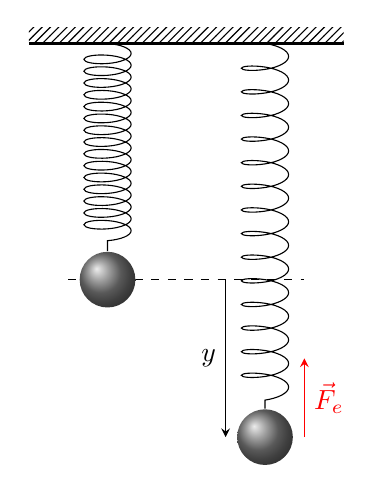
\begin{tikzpicture}
\draw[dashed] (-0.5,2) -- (2.5,2);
\draw[-stealth] (1.5,2) -- (1.5,0) node[midway, left] {$y$};
\draw[-stealth,red] (2.5,0) -- (2.5,1) node[midway, right] {$\vec{F}_e$};
\node[circle,ball color=gray,inner sep=2.5mm] (a) at (0,2) {};
\node[circle,ball color=gray,inner sep=2.5mm] (b) at (2,0) {};
\draw[decoration={aspect=0.3, segment length=3mm, amplitude=3mm,coil},decorate] (2,5) -- (b); 
\draw[decoration={aspect=0.3, segment length=1.5mm, amplitude=3mm,coil},decorate] (0,5) -- (a); 
\fill [pattern = north east lines] (-1,5) rectangle (3,5.2);
\draw[thick] (-1,5) -- (3,5);
\end{tikzpicture}
\caption{Sistema masa-resorte.}
\end{center}
\end{figure}\label{fig2.1}

La ecuación de movimiento que describe este sistema es

\begin{equation}
m\ddot{y}+ky=-mg,
\end{equation} \label{eq2.1}

que corresponde a un oscilador forzado, sin embargo, la solución particular a este problema corresponde a un desplazamiento del origen de coordenadas, por lo que será suficiente considerar la ecuación del oscilador armónico simple

\begin{equation}
m\ddot{y}+ky=0,
\end{equation} \label{eq2.2}

cuya solución se da en términos de funciones oscilatorias

\begin{equation}
y(t)=y_0\cos(\omega_0 t)
\end{equation} \label{eq2.3}

donde $\omega_0=\sqrt{k/m}$ es la frecuencia angular del sistema masa-resorte, a partir del cual se puede obtener el período $T=2\pi/\omega$. Supóngase que ahora la masa se sumerge en un fluido de viscosidad dinámica $\eta$ como se muestra en la figura \ref{fig2.2}. Aparece entonces un término adicional que responde por la fricción, y es proporcional a la velocidad y a la viscosidad del fluido $F_v=-\alpha\eta v$, donde $\alpha$ es una constante que depende de la geometría de la masa.

\begin{figure}
\begin{center}
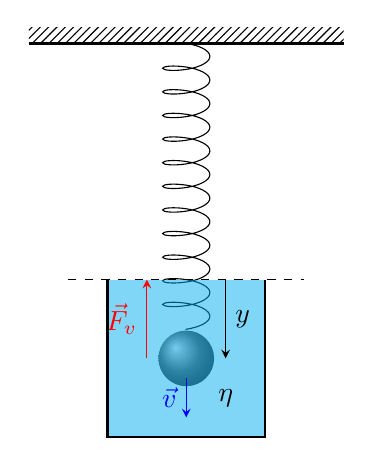
\begin{tikzpicture}
\draw[dashed] (-0.5,2) -- (2.5,2);
\node[circle,ball color=gray,inner sep=2.5mm] (a) at (1,1) {};
\draw[decoration={aspect=0.3, segment length=3mm, amplitude=3mm,coil},decorate] (1,5) -- (a); 
\fill [pattern = north east lines] (-1,5) rectangle (3,5.2);
\fill [cyan,opacity=0.5] (0,2) rectangle (2,0);
\draw[-stealth] (1.5,2) -- (1.5,1) node[midway, right] {$y$};
\draw[-stealth,red] (0.5,1) -- (0.5,2) node[midway, left] {$\vec{F}_v$};
\draw[-stealth,blue] (1,0.75) -- (1,0.25) node[midway, left] {$\vec{v}$};
\draw[thick] (-1,5) -- (3,5);
\draw[thick] (0,2) -- (0,0) -- (2,0) -- (2,2);
\node at (1.5,0.5) {$\eta$};
\end{tikzpicture}
\caption{Sistema masa-resorte en un líquido.}
\end{center}
\end{figure}\label{fig2.2}

Así entonces, la ecuación de movimiento del sistema es:

\begin{equation}
m\ddot{y}+\alpha\eta \dot{y}+ky=0
\end{equation}\label{eq2.4}

La solución de esta ecuación es también oscilatoria, sin embargo, su amplitud decrece exponencialmente con el tiempo

\begin{equation}
y(t)=y_0e^{-\frac{\gamma}{2}t}\cos(\omega t)
\end{equation}\label{eq2.5}

con $\gamma=\alpha\eta/m$ y $\omega=\sqrt{\omega_0^2-(\gamma/2)^2}$. De manera que conociendo el factor de amortiguamiento, se puede conocer la viscosidad del fluido.

\section{Desarrollo experimental}

Para el desarrollo experimental del proyecto se utilizaron cuatro resortes pequeños que fueron dispuestos en serie, de manera que forman un sistema con constante $k_{eq}$ definida por

\begin{equation}
k_{eq}=\dfrac{1}{\dfrac{1}{k_1}+\dfrac{1}{k_2}+\dfrac{1}{k_3}+\dfrac{1}{k_4}}.
\end{equation}\label{eq3.1}

Se dispuso también de dos masas: una de $32.46~\text{g}$ y otra de $99.00~\text{g}$, que se sujetan a los resortes; el sistema se pondrá a oscilar en el aire y en dos fluidos distintos: agua y aceite, y los datos serán tomados con ayuda de un circuito sencillo, compuesto de un sensor ultrasónico HC-SR04 \cite{datasheet} controlado por Arduino, específicamente con un ESP32, y serán subidas a una base de datos en Firebase, con el código mostrado en el anexo. La constante equivalente del sistema de resortes será determinada a través de la medición del período de oscilación en el aire del sistema con la masa de $99.00~\text{g}$, no será de interés encontrar las constantes individuales de cada resorte; mientras que la viscosidad del aceite relativa al agua será obtenida a partir de los coeficientes de amortiguamiento de los sistemas en las dos sustancias.\\

Una vez tenidos los datos, se procesan y ajustan usando \texttt{Python}, para obtener los parámetros físicos de interés en el sistema.

\section{Resultados}

Los datos almacenados en la base de datos se exportaron como archivo \texttt{.json}, que es apto para lectura en \texttt{Python} a través de la librería \texttt{pandas}, para ser procesados y ajustados de acuerdo a las ecuaciones \ref{eq2.3} y \ref{eq2.5}, según sea el caso, obteniendo las siguientes curvas:

\begin{figure}[h!]
\begin{center}
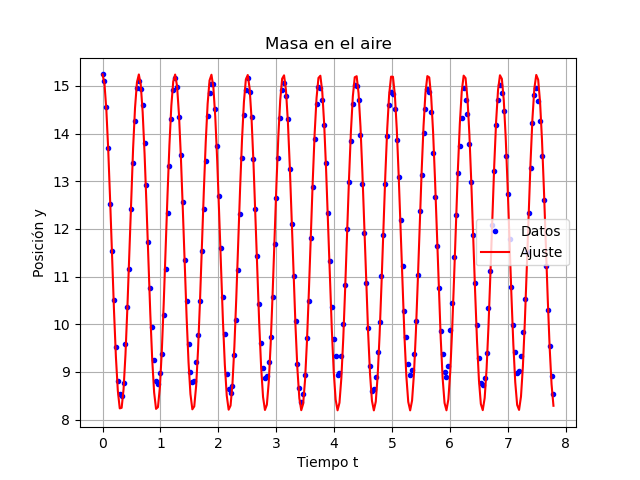
\includegraphics[width=\columnwidth]{../aire.png} 
\end{center}
\caption{Movimiento de la masa en el aire.}
\end{figure}\label{fig4.1}

\begin{figure}[h!]
\begin{center}
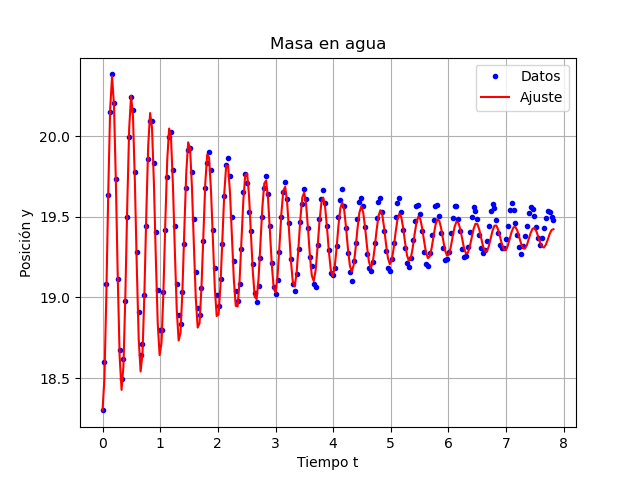
\includegraphics[width=\columnwidth]{../agua.png} 
\end{center}
\caption{Movimiento de la masa en el agua.}
\end{figure}\label{fig4.2}

\begin{figure}[h!]
\begin{center}
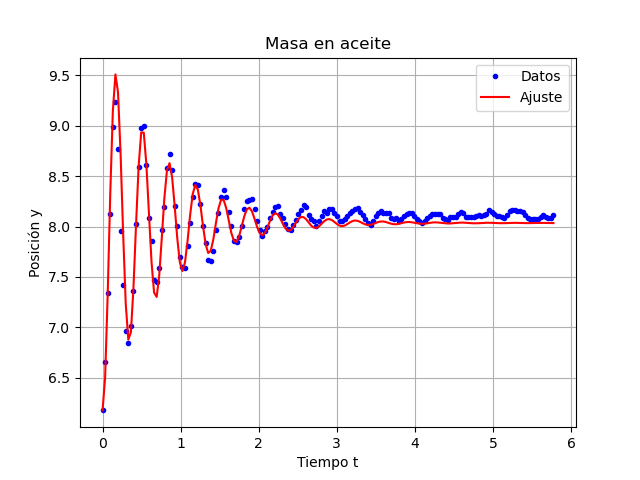
\includegraphics[width=\columnwidth]{../aceite.png} 
\end{center}
\caption{Movimiento de la masa en el aceite.}
\end{figure}\label{fig4.3}

Los parámetros de ajuste relevantes para este trabajo son la constante $k$ del sistema de resortes y los coeficientes de amortiguamiento, que dentro del ajuste están representados por $C=m\gamma$. Se tomó como referencia el aire para calcular la constante del sistema de resortes, dando un valor de:

\begin{equation}
k=(10008\pm 4)~\text{g/s}^2
\end{equation}\label{eq4.1}

De los movimientos amortiguados se obtienen los valores de $C$, que está relacionada con la viscosidad de los medios a través de la relación con $\gamma$, dando los siguientes valores:

\begin{align}
C_w = (24.5\pm0.6)~\text{g/s}\\
C_o = (86\pm3)~\text{g/s}
\end{align}\label{eq4.2}

Donde $C_w$ es el parámetro de amortiguamiento del agua y $C_o$ es el mismo parámetro de amortiguamiento del aceite. Sin ambargo, como el coeficiente de amoritugamiento contiene un factor $\alpha$ que depende de la geometría de la masa, de modo que si se quiere conocer cuál es la viscosidad del medio, debería conocerse el valor de $\alpha$. Se puede en su lugar, encontrar la viscosidad del aceite relativa a la del agua, para poder ser comparada así con los valores reportados en la literatura. Así entonces, la viscosidad relativa $\eta_R$ es:

\begin{equation}
\eta_R=\dfrac{C_o}{C_w}=3.54\pm0.04
\end{equation}\label{eq4.3}

En la literatura se reporta un valor de $10^{-3}~\text{Pa}\cdot\text{s}$ \cite{kestin1978viscosity} para la viscosidad del agua, mientras que para el aceite de girasol, que fue el utilizado en este experimento, es de $0.0488~\text{Pa}\cdot\text{s}$; de modo que la viscosidad del aceite relativa al agua es dada por el cociente entre estas dos cantidades: $m$

\bibliographystyle{abbrv} 
\bibliography{example.bib}

%% else use the following coding to input the bibitems directly in the
%% TeX file.

%%\begin{thebibliography}{00}

%% \bibitem[Author(year)]{label}
%% For example:

%% \bibitem[Aladro et al.(2015)]{Aladro15} Aladro, R., Martín, S., Riquelme, D., et al. 2015, \aas, 579, A101


%%\end{thebibliography}

\end{document}

\endinput
%%
%% End of file `elsarticle-template-harv.tex'.
